% =============================================================================
% CAPÍTULO 7 — volta 4 (AGENTS.md §6): ver mundos basta, ou é preciso mexer no mundo?
%
% O fracasso que o abre, com número na mão: acumular mercados não faz a região encolher. Os três
% entregam a mesma margem (a taxa vai de 0,0509 a 0,0520) e discordam do agrupamento (o pior
% bloco vai de 14 a 20); sozinhos admitem 0, 3 e 14 explicações, e a interseção é vazia.
%
% Medição: lab/experimentos/E08_observar_ou_intervir.ipynb. Figuras: figuras/E08_observar_ou_intervir_*.
% =============================================================================

\chapter{Ver mundos basta}
\label{cap:observar}

\section{A tentativa de sempre}

O capítulo anterior deixou uma região: quatro estatísticas medidas num mercado não escolhem uma
explicação entre as duas que sobreviveram, e encolher a região com mais estatística tem limite,
porque todas elas vêm do mesmo pedaço de passado. A saída que se oferece sozinha é acumular
mundos. Mais mercados, mais períodos, mais domínios --- e o que era indistinguível num deles fica
separado pelo conjunto.

A tentativa tem uma forma precisa, e vale escrevê-la: o mecanismo é o mesmo em toda parte, e cada
mercado só tem a sua escala. Se for assim, observar mais mundos identifica o mecanismo, e a
intervenção deixa de ser necessária. Este capítulo mede se é assim, com \numObservarMercados{}
mercados no lugar de um.

O primeiro mercado é o de sempre, com \numObservarDiasMaior{} dias. Os outros dois são o índice
brasileiro e o bitcoin, e o empréstimo fica declarado: os três atravessam do arquivo do projeto
anterior, e todo número tirado deles é medido de novo aqui.

\section{O que os três concordam}

A promessa do primeiro capítulo --- a linha no décimo terceiro pior dos últimos
\numCorteJanela{} pregões --- aplicada aos três mercados, entrega a mesma coisa em todos. A taxa
de rompimento vai de \numObservarTaxaMenor\% a \numObservarTaxaMaior\%, e a distância entre os dois
extremos é de um décimo de ponto percentual.

Isso não é acidente. É a proposição da conta do corte funcionando três vezes: o corte assina a
média, e assina a mesma média em qualquer série, porque a conta é do corte e não do mundo. O que
a leitura acrescenta é que a margem dos três mercados é a mesma coisa --- a oscilação de um dia
para o outro tem a mesma forma nos três, e o que muda entre eles é o tamanho, não o desenho.

Onde os três se separam é no agrupamento. O pior bloco de sessenta dias vai de
\numObservarPiorMenor{} a \numObservarPiorMaior{} rompimentos, e essa distância é grande. A
margem concorda; a forma com que os dias ruins se juntam, não.

\section{O que os três discordam}

A conta é a do capítulo anterior, feita três vezes: uma família de explicações --- duas leis, uma
calma e uma agitada, com o estado durando ---, e quatro estatísticas medidas em cada mercado. Uma
explicação serve a um mercado quando reproduz as quatro dentro da tolerância.

O primeiro mercado admite \numObservarSobreviventesIndice{} explicações. O segundo admite
\numObservarSobreviventesIbov. O terceiro admite \numObservarSobreviventesBitcoin. Ao todo,
\numObservarUniao{} explicações sobrevivem em algum deles.

Quantas sobrevivem aos três, ao mesmo tempo, é o número deste capítulo:
\numObservarIntersecao.

\begin{figure}[htbp]
  \centering
  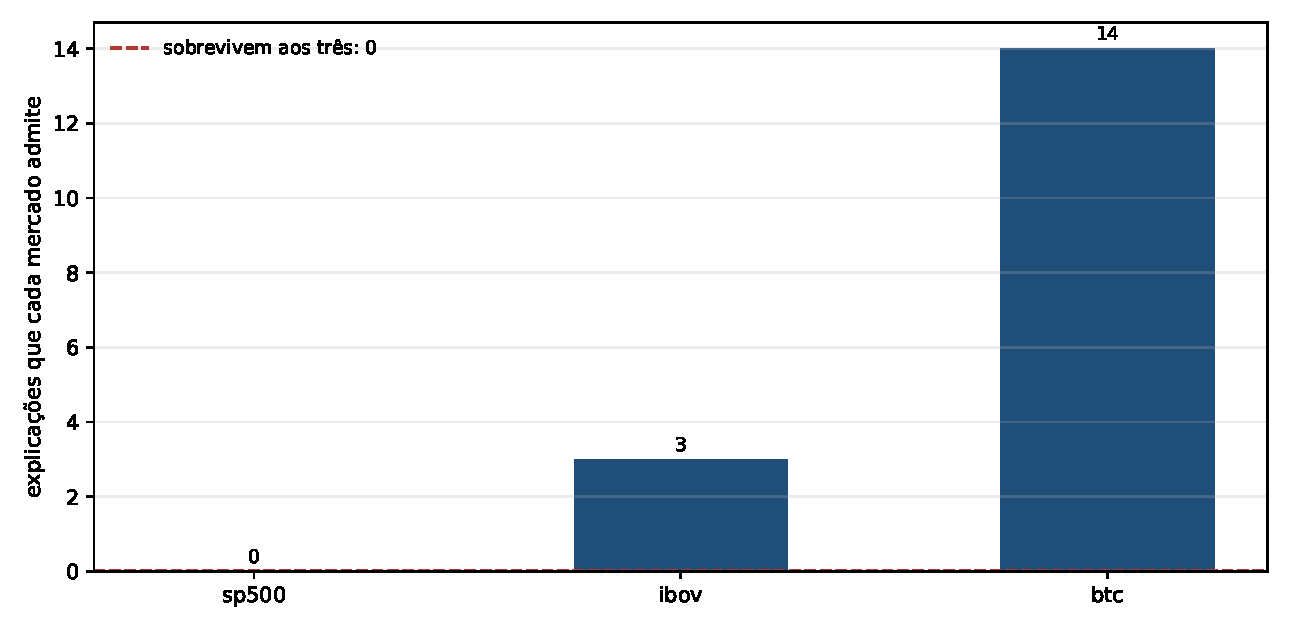
\includegraphics[width=0.8\linewidth]{figuras/E08_observar_ou_intervir_1.pdf}
  \caption{Quantas explicações cada mercado admite sozinho, e a linha da interseção. A primeira
    barra não aparece porque o valor dela é o zero: o mercado com mais dados é o que não admite
    explicação nenhuma. Barra ausente e barra que faltou têm a mesma cara, e a linha colada no
    eixo some.}
  \label{fig:admite}
\end{figure}

Acumular mundos não fez a região encolher para uma resposta. Fez os mundos discordarem.

\section{Com a lei compartilhada}

Vale abrir a porta que a seção anterior deixou entreaberta. A conta admitia que cada mercado
tivesse os seus próprios parâmetros, e discordar assim é fácil: séries diferentes têm números
diferentes. A pergunta dura é se eles discordam do **mecanismo**, e para isso a lei passa a ser
compartilhada: um único triplo de parâmetros governa os três, e cada mercado conserva apenas a sua
escala.

A grade grossa tem \numObservarCombinacoes{} triplos, e \numObservarGrossa{} deles servem aos três
mercados. A grade fina tem \numObservarTriplosFinos, e \numObservarFina{} deles servem. As duas
contas dão o mesmo vazio, e a segunda existe para que a conclusão não seja da malha: escolha de
quem mede não pode decidir o resultado.

A discordância, então, é do mecanismo e não do tamanho. E ela tem uma estatística preferida, que
a seção seguinte isola.

\section{Qual estatística é o gargalo}

Num conjunto vazio, a pergunta útil é de onde vem o vazio. Das quatro estatísticas, quantas são
satisfeitas pelos três mercados ao mesmo tempo, no mesmo triplo de parâmetros?

\begin{table}[htbp]
  \centering
  \begin{tabular}{lr}
    \hline
    estatística & triplos que servem aos três \\
    \hline
    a mediana dos blocos & \numObservarNosTresMediana \\
    a taxa de rompimento & \numObservarNosTresTaxa \\
    o excesso de blocos cheios & \numObservarNosTresExcesso \\
    o pior bloco de sessenta dias & \numObservarNosTresPior \\
    \hline
  \end{tabular}
  \caption{Dos \numObservarTriplosFinos{} triplos da grade fina, quantos satisfazem cada
    estatística nos três mercados simultaneamente.}
  \label{tab:gargalo}
\end{table}

A mediana é satisfeita por todos, e isso não é mérito: o valor dela é dois ou três em toda parte,
e uma estatística grosseira não separa nada. A taxa vai longe, porque é a margem --- e a margem
concorda. O gargalo é o \textbf{pior bloco}: só \numObservarNosTresPior{} triplos de
\numObservarTriplosFinos{} conseguem reproduzir, nos três mercados ao mesmo tempo, o agrupamento
dos dias ruins.

É o mesmo gargalo do capítulo anterior, olhado de outro lado. Lá ele esvaziava uma família dentro
de um mercado; aqui, ele separa os mercados entre si.

\section{A tentativa de consertar, e o que ela ensinou}

Resta a hipótese mais generosa: a família é pobre na dimensão do agrupamento, e enriquecê-la
resolve. Ela foi enriquecida --- a duração média dos episódios de agitação deixou de ser uma só, e
cada episódio passou a sortear a sua entre uma curta e uma longa.

A taxa de acerto diz o contrário. Com a duração única, a família reproduz as duas estatísticas de
agrupamento em \numObservarAcertoUnicaIndicePct\% das tentativas no primeiro mercado,
\numObservarAcertoUnicaIbovPct\% no segundo e \numObservarAcertoUnicaBitcoinPct\% no terceiro. Com a
duração heterogênea, os mesmos três números caem para \numObservarAcertoHeteroIndicePct\%,
\numObservarAcertoHeteroIbovPct\% e \numObservarAcertoHeteroBitcoinPct\%.

Enriquecer exatamente a dimensão que discordava não consertou nada: piorou. E há uma lição de
método embutida nessa tabela, que este livro já pagou uma vez. A primeira versão desta varredura
usou uma semente por configuração, e a mesma configuração deu pior bloco de quinze a dezenove em
cinco sementes --- variação maior que qualquer diferença entre configurações. O veredito acima só
existe porque a conta foi refeita com quarenta sementes em cada célula, reportando mediana e
dispersão. \textbf{Toda medição sobre mundos sorteados reporta dispersão, ou não reporta nada.}

\begin{figure}[htbp]
  \centering
  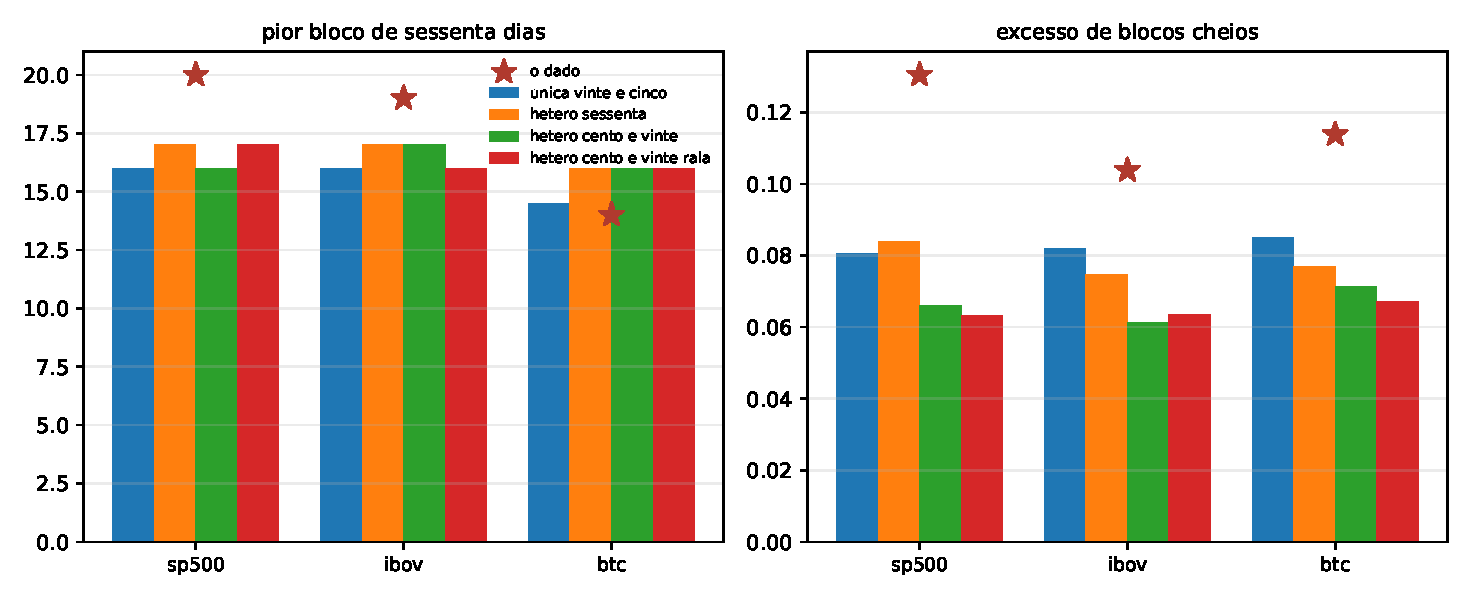
\includegraphics[width=\linewidth]{figuras/E08_observar_ou_intervir_2.pdf}
  \caption{A mediana do pior bloco e a do excesso, por configuração e por mercado, com o valor do
    dado como estrela. As barras são medianas e as estrelas são pontos, sem dispersão desenhada:
    as faixas de dez a noventa por cento se sobrepõem, de modo que a distância aparente entre
    barra e estrela é maior do que a distância entre as distribuições.}
  \label{fig:replicacao}
\end{figure}

\section{O que fica}

Fica a resposta, provisória e por eliminação. Acumular mundos não identificou um mecanismo
comum. As marginais dos três mercados concordam --- a promessa do primeiro capítulo é cumprida
três vezes, com a mesma conta e o mesmo número ---, e o agrupamento discorda, com o gargalo
isolado na estatística que mede como os dias ruins se juntam. Com a lei compartilhada o vazio
continua, nas duas malhas; enriquecendo a duração dos episódios, piora.

A resposta é provisória porque uma porta fica declarada aberta, e fechá-la seria afirmar mais do
que foi medido: uma família **mais rica** --- memória longa além de troca de regimes, parâmetros
que variam no tempo --- ainda não foi testada, e é o único caminho que mantém vivo o refutador
desta pergunta. O que está medido, e é o que o capítulo assina, é mais estreito e ainda assim
forte: na família que este livro sabe construir, **ver mundos não basta**.

O que sobra é a intervenção, e com ela o fracasso seguinte. Não basta querer intervir: é preciso
dizer que intervenção distinguiria as duas explicações que sobreviveram no primeiro mercado, e
quanto ela custaria em dado que não existe. Um experimento que não se pode fazer é uma opinião com
instrumentos; um que se pode fazer é uma medida, e é essa diferença que a travessia deste livro
ainda tem de enfrentar.
